
\noindent \textcolor{COLOR2}{RESULTADOS}
\\

\begin{table}[ht]
    \label{tab:resultados}
    \centering
    \begin{tabular}{lc}
        \rowcolor{pagecolor!50!COLOR1}
        \hline
        Modelo & Acurácia (ACC) \\\hline\hline
        LR     & 0.774603       \\\hline
        LDA    & 0.785516       \\\hline
        KNN    & 0.766865       \\\hline
        CART   & 0.681746       \\\hline
        NB     & 0.790278
    \end{tabular}
    \caption{Comparação inicial entre modelos}
\end{table}

A partir de agora, a fim de facilitar a escrita e compreensão, denominar-se-á como:

\begin{itemize}
    \item \textcolor{deepblue}{LDA} - Análise discriminante;
    \item \textcolor{deepblue}{LR} - Regressão Logística;
    \item \textcolor{deepblue}{KNN} - K-ésimo Vizinho mais Próximo;
    \item \textcolor{deepblue}{CART} - Árvore de decisão;
    \item \textcolor{deepblue}{NB} - Naive Bayes;
\end{itemize}

Em primeira mão, analisou-se os modelos com os conjuntos de treinamento para verificar qual deles aparesentaria a \textit{priori} a melhor precisão. Por se tratar de uma comparação entre os modelos, utilizou-se a métrica de acurácia (ACC) para fazer essa avaliação. O Resultado obtido é dado na tabela \pageref{tab:resultados}.\\

É possível observar pela validação cruzada (Kfold) que o modelo NB apresenta a maior acurácia, com um valor de 0.790278 e o CART o menor com um valor de 0.681746. Verificar-se-á com a execução dos modelos se esse resultado é de fato o encontrado.
\\

\noindent \textcolor{deepblue}{1) LDA - ANÁLISE DISCRIMINANTE}

\begin{figure}[ht]
    \centering
    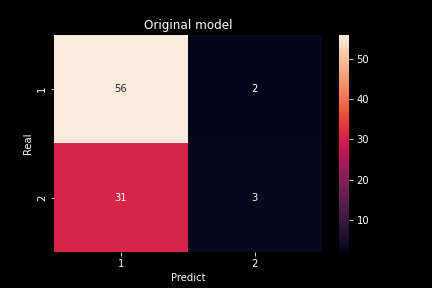
\includegraphics[width=\linewidth, scale=.6]{../../figuras/machine_learning/LDA_MC.png}
    \caption{Matriz de confusão da Análise discriminante}
\end{figure}

